\documentclass[a4paper, 14pt]{extarticle}
\usepackage[utf8]{inputenc}
\usepackage[paper=a4paper, top=1cm, right=1cm, bottom=1.5cm, left=2cm]{geometry}
\usepackage{setspace}
\onehalfspacing

\usepackage{graphicx}
\graphicspath{{plots/}, {images/}}

\parindent=1.25cm

\usepackage{titlesec}

\titleformat{\section}
    {\normalsize\bfseries}
    {\thesection}
    {1em}{}

\titleformat{\subsection}
    {\normalsize\bfseries}
    {\thesubsection}
    {1em}{}

% Настройка вертикальных и горизонтальных отступов
\titlespacing*{\chapter}{0pt}{-30pt}{8pt}
\titlespacing*{\section}{\parindent}{*4}{*4}
\titlespacing*{\subsection}{\parindent}{*4}{*4}

\usepackage[square, numbers, sort&compress]{natbib}
\makeatletter
\bibliographystyle{unsrt}
\renewcommand{\@biblabel}[1]{#1.} 
\makeatother


\newcommand{\maketitlepage}[6]{
    \begin{titlepage}
        \singlespacing
        \newpage
        \begin{center}
            Министерство образования и науки Российской Федерации \\
            Федеральное государственное бюджетное образовательное \\
            учреждение высшего профессионального образования \\
            <<Волгоградский государственный технический университет>> \\
            #1 \\
            Кафедра #2
        \end{center}


        \vspace{14em}

        \begin{center}
            \large Семестровая работа #6 по дисциплине
            \\ <<#3>>
        \end{center}

        \vspace{5em}

        \begin{flushright}
            \begin{minipage}{.35\textwidth}
                Выполнила:\\#4
                \vspace{1em}\\
                Проверил:\\#5
                \\
                \\ Оценка \underline{\ \ \ \ \ \ \ \ \ \ \ \ \ \ \ \ }
            \end{minipage}
        \end{flushright}

        \vspace{\fill}

        \begin{center}
            Волгоград, \the\year
        \end{center}

    \end{titlepage}
    \setcounter{page}{2}
}

\newcommand{\maketitlepagewithvariant}[7]{
    \begin{titlepage}
        \singlespacing
        \newpage

        \begin{center}
            Министерство образования и науки Российской Федерации \\
            Федеральное государственное бюджетное образовательное \\
            учреждение высшего профессионального образования \\
            <<Волгоградский государственный технический университет>> \\
            #1 \\
            Кафедра #2
        \end{center}


        \vspace{8em}

        \begin{center}
            \large Семестровая работа #6 по дисциплине
            \\ <<#3>>
        \end{center}

        \vspace{1em}
        \begin{center}
            Вариант №#7
        \end{center}
        \vspace{4em}

        \begin{flushright}
            \begin{minipage}{.35\textwidth}
                Выполнила:\\#4
                \vspace{1em}\\
                Проверил:\\#5
                \\
                \\ Оценка \underline{\ \ \ \ \ \ \ \ \ \ \ \ \ \ \ \ }
            \end{minipage}
        \end{flushright}

        \vspace{\fill}

        \begin{center}
            Волгоград, \the\year
        \end{center}

    \end{titlepage}
    \setcounter{page}{2}
}

\input{../../.preambles/10-russian}
\input{../../.preambles/20-math}

\newcolumntype{L}[1]{>{\flushleft\arraybackslash}m{#1\textwidth}}

\begin{document}
\maketitlepage{Факультет электроники и вычислительной техники}{физики}
{Специальные функции}{студент группы Ф-369\\Чечеткин~И.~А.}
{к.~ф.-м.~н., доцент\\Никулин~Р.~Н.}{\!\!}

\begin{table}[h!]
    \center
    \begin{tabular}{m{.75\textwidth}C{.15}}
    №17. Дана тяжелая однородная тонкая нить длины \( l \). Нить закреплена верхним
    концом в точке \( x = l \) и совершает колебания под действием силы тяжести.
    Максимальное отклонение ее нижнего конца \( x = 0 \) по вертикали равно \( h \).
    За ось \( х \) примем вертикальное направление, вдоль которого расположится
    нить, когда под действием своего веса она займет прямолинейное положение.
    Обозначим через \( u = u(x, t) \) отклонение точек нити от положения равновесия
    в момент времени \( t \) (см. рис). Рассматривая малые колебания нити такие, что
    можно пренебречь величиной \( \left(\pder{u}{x}\right)^2 \) по сравнению с
    единицей, найти выражение для \( u(x, t) \).
    
    [Найти \( u(x, t)\).] &
    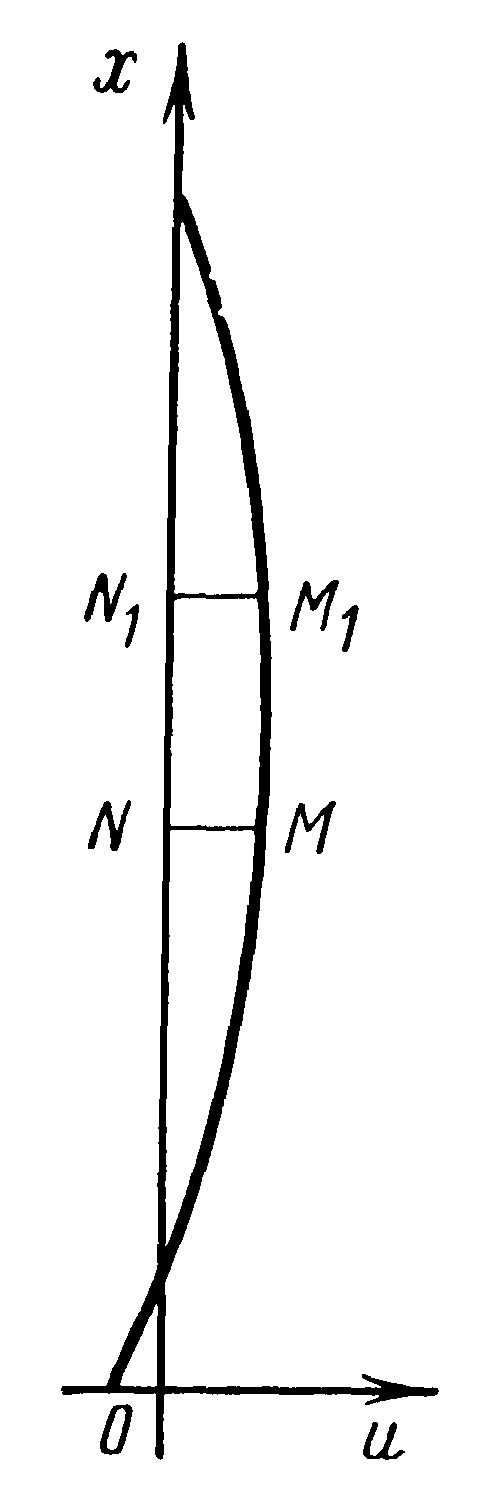
\includegraphics[width=.13\textwidth]{scheme}
    \end{tabular}
\end{table}

\vspace*{2em}
\emph{Решение}. Так как рассматриваются малые колебания, то:
\begin{align*}
    & \sin\alpha(x) = \frac{\tg\alpha(x)}{\sqrt{1 + \tg^2\alpha(x)}} =
    \frac{\pder{u}{x}}{\sqrt{1 + \left(\pder{u}{x}\right)^2}} \approx \pder{u}{x}, \\
    & \cos\alpha(x) = \frac{1}{\sqrt{1 + \tg^2\alpha(x)}} =
    \frac{1}{\sqrt{1 + \left(\pder{u}{x}\right)^2}} \approx 1,
\end{align*}
где \( \alpha(x) \) --- угол между касательной в точке с абсциссой \( x \) к нити в момент
времени \( t \) и положительным направлением оси \( Ox \).

Натяжение \( T \) нити в точке \( N \) с абсциссой \( x \) равно весу
части нити, расположенной вниз от \( N \), т. е. \( T = g\rho x \), где \( \rho \) --- линейная
плотность нити, a \( g \) --- ускорение силы тяжести.

Выделим произвольный элемент нити \( MM_1 \), длиной \( \d x \), который при
равновесии занимал положение \( NN_1 \) (см. рис). Горизонтальная составляющая
равнодействующей сил натяжения, действующих на концы элемента \( MM_1 \),
выражается разностью
\[
    T_H = \left(g\rho x\pder{u}{x}\right)_{M_1} - \left(g\rho x\pder{u}{x}\right)_M,
\]
которая с точностью до бесконечно малых высшего порядка равна выражению
\[
    T_H = g\rho\pder{}{x}\left(x\pder{u}{x}\right)\d x.
\]

Вертикальная составляющая равна
\[
    T_V = (g\rho x\cos\alpha(x))_{M_1} - (g\rho x\cos\alpha(x))_M \approx g\rho\d x.
\]

Отсюда видно, что вертикальная составляющая равнодействующей сил натяжения
и сила тяжести, равная \( g\rho\d x \) и направленная вниз, взаимно уничтожаются.
Поэтому можно считать, что элемент нити \( MM_1 \) движется под действием
только горизонтальной составляющей силы \( T_H \). Тогда
искомое дифференциальное уравнение малых колебаний подвешенной нити:
\begin{equation}
    \pder{}{x}\left(x\pder{u}{x}\right) = \frac{1}{g}\ppder{u}{t}.
    \label{eq:equation}
\end{equation}
Задача о колебании подвешенной нити сводится к интегрированию уравнения
\eqref{eq:equation} с граничным условием
\begin{equation}
    u|_{x = l} = 0
    \label{condition_corner}
\end{equation}
и с начальными условиями
\begin{equation}
    u|_{t = 0} = f(x), \hspace{2em} \left.\pder{u}{t}\right|_{t = 0} = F(x).
    \label{condition_zero}
\end{equation}

Чтобы применить метод разделения переменных преобразуем уравнение
\eqref{eq:equation} к новой переменной \( \xi = \sqrt{x} \), тогда преобразованное
уравнение примет вид:
\begin{equation}
    \frac{1}{4\xi}\pder{}{\xi}\left(\xi\pder{u}{\xi}\right) = \frac{1}{g}\ppder{u}{t}.
    \label{eq:eq_xi}
\end{equation}

Будем искать решение уравнения в виде \eqref{eq:solve_type}:
\begin{equation}
    u = v(\xi)T(t).
    \label{eq:solve_type}
\end{equation}

Подставляя \eqref{eq:solve_type} в \eqref{eq:eq_xi}, получим следующее:
\[
    \frac{1}{\xi v}\der{}{\xi}\left(\xi\der{v}{\xi}\right) = \frac{4}{g}\frac{1}{T}\dder{T}{t}.
\]
Обозначая обе части равенства через постоянную \( -\lambda^2 \), получим два
уравнения:
\begin{align}
    & \der{}{\xi}\left(\xi\der{v}{\xi}\right) + \lambda^2\xi v = 0, \label{eq:v_xi} \\
    & \dder{T}{t} + g\left(\frac{\lambda}{2}\right)^2T = 0. \label{eq:T_t}
\end{align}

Уравнение \eqref{eq:v_xi} является уравнением Бесселя, общее решение которого
можно представить в виде
\begin{equation}
    v(\xi) = C_1J_0(\lambda\xi) + C_2Y_0(\lambda\xi),
    \label{eq:v_common}
\end{equation}
где \( J_0(\lambda\xi) \) -- функция Бесселя первого рода нулевого порядка:
\[
    J_0(\lambda\xi) =
    \sum\limits_{k = 0}^\infty \frac{(-1)^k\left(\frac{\lambda\xi}{2}\right)^{2k}}
    {k!\Gamma(k + 1)};
\]
а \( Y_0(\lambda\xi) \) -- функция Бесселя второго рода нулевого порядка:
\[
    Y_0(\lambda\xi) = \frac{2}{\pi}J_0(\lambda\xi)\ln\frac{\lambda\xi}{2} - \frac{2}{\pi}
    \sum\limits_{k = 0}^\infty \frac{(-1)^k\left(\frac{\lambda\xi}{2}\right)^{2k}}{(k!)^2}
    \frac{\Gamma'(k+1)}{\Gamma(k+1)}.
\]
Так как при \( \xi \to 0 \) значение \( |Y_0(\lambda\xi)| \to \infty \), то постоянную \( C_2 \)
в уравнении \eqref{eq:v_common} приравниваем к нулю. Тогда граничное условие
\eqref{condition_corner} даст
\[
    J_0(\lambda\sqrt{l}) = 0.
\]
Уравнение \( J_0(\mu) = 0 \) имеет бесчисленное множество вещественных корней:
\( \mu_1 \),~\( \mu_2 \),~\ldots Отсюда вытекает, что собственные числа задачи
определяются равенством
\begin{equation}
    \lambda_k^2 = \frac{\mu_k^2}{l}, \hspace{1em} k = 1, 2, 3, \ldots
    \label{own_nums}
\end{equation}

Следовательно, собственные функции, соответствующие этим собственным числам
имеют следующий вид:
\[
    v_k(x) = J_0\left(\mu_k\sqrt{\frac{x}{l}}\right).
\]

Общее решение уравнения \eqref{eq:T_t} с учетом \eqref{own_nums} имеет вид:
\[
    T_k(t) = A_k\cos\frac{\sqrt{g}\mu_kt}{2\sqrt{l}} + B_k\sin\frac{\sqrt{g}\mu_kt}{2\sqrt{l}}.
\]
Следовательно, ряд \eqref{eq:row_solve}
\begin{equation}
    u(x, t) = \sum\limits_{k = 1}^\infty \left(A_k\cos\frac{\sqrt{g}\mu_kt}{2\sqrt{l}} +
    B_k\sin\frac{\sqrt{g}\mu_kt}{2\sqrt{l}}\right)J_0\left(\mu_k\sqrt{\frac{x}{l}}\right)
    \label{eq:row_solve}
\end{equation}
даст решение уравнения \eqref{eq:equation} при граничном условии
\eqref{condition_corner}.

Положив в разложении \eqref{eq:row_solve} \( t = 0 \), получим, что
\[
    f(x) = \sum\limits_{k = 1}^\infty A_k J_0\left(\mu_k \sqrt{\frac{x}{l}} \right).
\]
Это выражение является разложением функции \( f(x) \) в ряд Фурье--Бесселя. Тогда
коэффициенты \( A_k \) выражаются следующим образом:
\[
    A_k = \frac{1}{l J_1^2(\mu_k)} \int\limits_0^l f(x)J_0\left(\mu_k\sqrt{\frac{x}{l}}\right)\d x.
\]
Взяв производную от разложения \eqref{eq:row_solve} и рассуждая аналогичным
образом, найдем коэффициенты \( B_k \):
\[
    B_k = \frac{2}{\sqrt{gl}\mu_k J_1^2(\mu_k)} \int\limits_0^l F(x)J_0
    \left(\mu_k\sqrt\frac{x}{l}\right)\d x.
\]

Обозначая \( A_k = N_k\sin\phi_k \), \( B_k = N_k\cos\phi_k \), перепишем
\eqref{eq:row_solve} в форме:
\begin{equation}
    u(x, t) = \sum\limits_{k = 1}^\infty N_k J_0\left(\mu_k\sqrt{\frac{x}{l}}\right)
    \sin\left(\frac{\sqrt{g}\mu_kt}{2\sqrt{l}} + \phi_k\right).
    \label{eq:final_solve}
\end{equation}

Отсюда видно, что малые колебания подвешенной нити можно рассматривать
как движение, складывающееся из бесчисленного множества гармонических
колебаний.

\newpage
\addcontentsline{toc}{section}{Список литературы}
\begin{thebibliography}{9}
    \bibitem{Koshljakov}Кошляков,~Н.~С. Уравнения в частных производных
    математической физики [Текст] / Кошляков~Н.~С., Глинер~Е.~Б., Смирнов~М.~М.
    Учебное пособие. -- М.: <<Высшая школа>>, 1970.-- 712с.
\end{thebibliography}
\end{document}